%%%%%%%%%%%%%%%%%%%%%%%%%%%%%%%%%%%%%%%%%
% Beamer Presentation
% LaTeX Template
% Version 1.0 (10/11/12)
%
% This template has been downloaded from:
% http://www.LaTeXTemplates.com
%
% License:
% CC BY-NC-SA 3.0 (http://creativecommons.org/licenses/by-nc-sa/3.0/)
%
%%%%%%%%%%%%%%%%%%%%%%%%%%%%%%%%%%%%%%%%%

%----------------------------------------------------------------------------------------
%	PACKAGES AND THEMES
%----------------------------------------------------------------------------------------

\documentclass{beamer}
\usepackage{subfig}
\usepackage{pgfplots}

\mode<presentation> {

% The Beamer class comes with a number of default slide themes
% which change the colors and layouts of slides. Below this is a list
% of all the themes, uncomment each in turn to see what they look like.

%\usetheme{default}
%\usetheme{AnnArbor}
%\usetheme{Antibes}
%\usetheme{Bergen}
%\usetheme{Berkeley}
%\usetheme{Berlin}
%\usetheme{Boadilla}
%\usetheme{CambridgeUS}
%\usetheme{Copenhagen}
%\usetheme{Darmstadt}
%\usetheme{Dresden}
%\usetheme{Frankfurt}
%\usetheme{Goettingen}
%\usetheme{Hannover}
%\usetheme{Ilmenau}
%\usetheme{JuanLesPins}
%\usetheme{Luebeck}
\usetheme{Madrid}
%\usetheme{Malmoe}
%\usetheme{Marburg}
%\usetheme{Montpellier}
%\usetheme{PaloAlto}
%\usetheme{Pittsburgh}
%\usetheme{Rochester}
%\usetheme{Singapore}
%\usetheme{Szeged}
%\usetheme{Warsaw}

% As well as themes, the Beamer class has a number of color themes
% for any slide theme. Uncomment each of these in turn to see how it
% changes the colors of your current slide theme.

%\usecolortheme{albatross}
%\usecolortheme{beaver}
%\usecolortheme{beetle}
%\usecolortheme{crane}
%\usecolortheme{dolphin}
%\usecolortheme{dove}
%\usecolortheme{fly}
%\usecolortheme{lily}
%\usecolortheme{orchid}
%\usecolortheme{rose}
%\usecolortheme{seagull}
%\usecolortheme{seahorse}
%\usecolortheme{whale}
%\usecolortheme{wolverine}

%\setbeamertemplate{footline} % To remove the footer line in all slides uncomment this line
%\setbeamertemplate{footline}[page number] % To replace the footer line in all slides with a simple slide count uncomment this line

%\setbeamertemplate{navigation symbols}{} % To remove the navigation symbols from the bottom of all slides uncomment this line
}

\usepackage{graphicx} % Allows including images
\usepackage{booktabs} % Allows the use of \toprule, \midrule and \bottomrule in tables

%----------------------------------------------------------------------------------------
%	TITLE PAGE
%----------------------------------------------------------------------------------------

\title[Fashion recommender systems]{Fashion recommender systems with focus on time and 
        seasonability} % The short title appears at the bottom of every slide, the full title is only on the title page

\author{Jaime Ferrando Huertas} % Your name
% \institute[H\&M] % Your institution as it will appear on the bottom of every slide, may be shorthand to save space
{

\medskip
% \textit{john@smith.com} % Your email address
}
\date{\today} % Date, can be changed to a custom date

\begin{document}

\begin{frame}
\titlepage % Print the title page as the first slide
\end{frame}

\begin{frame}
\frametitle{Overview} % Table of contents slide, comment this block out to remove it
\tableofcontents % Throughout your presentation, if you choose to use \section{} and \subsection{} commands, these will automatically be printed on this slide as an overview of your presentation
\end{frame}

%----------------------------------------------------------------------------------------
%	PRESENTATION SLIDES
%----------------------------------------------------------------------------------------

%------------------------------------------------
\section{Introduction} % Sections can be created in order to organize your presentation into discrete blocks, all sections and subsections are automatically printed in the table of contents as an overview of the talk
%------------------------------------------------
\begin{frame}{Introduction}
\begin{columns}[c] % The "c" option specifies centered vertical alignment while the "t" option is used for top vertical alignment

\column{.65\textwidth} % Left column and width
\begin{itemize}
\item Master Thesis collaboration with H\&M.
\item 40\% increase in online revenue from 2019 to 2020, with a total of 5.1 Billion euros. Highly susceptible for improvements on recommender systems
\item Fashion industry - different scenario as seen in state of the art recommender systems.
\end{itemize}

\column{.3\textwidth} % Right column and width 
\begin{figure}%
    \centering
    \centering{{
\includegraphics[scale=0.07]{images/1200px-H&M-Logo.svg.png} }}%
    % \caption{2 Figures side by side}%
\end{figure}
\end{columns}
\end{frame}

\begin{frame}{Introduction - Research question}

\begin{itemize}
\item Does treating our user's history as an ordered sequenced of events improve our recommendation models?
\end{itemize}
\end{frame}

\begin{frame}{Introduction - State of the art}

\begin{figure}[!htb]
\minipage{0.25\textwidth}
  
\includegraphics[width=\linewidth, scale=0.3]{images/spotifylogo.png}
\endminipage\hfill
\minipage{0.32\textwidth}
  
\includegraphics[width=\linewidth]{images/youtubelogo.png}
\endminipage\hfill
\minipage{0.32\textwidth}%
  
\includegraphics[width=\linewidth]{images/ALIBABA-LOGO.png}
\endminipage
\end{figure}
\begin{itemize}
\item Usage of Deep Learning methods across big tech companies. Models very closed to what is used in NLP.
\end{itemize} 

\end{frame}

\section{Dataset}
\begin{frame}{Dataset - Google anaylicts data}
\begin{itemize}
    \item User interactions in H\&M website. Clicks, views.
    \item Swedish Market
    \item Between 2021-03-01 and 2021-04-01
    \item Last user interactions as test set.
\end{itemize}
\end{frame}

\begin{frame}{Dataset - Preprocessing}
Given a user history $H$ containing $h_1, h_2, .. h_n$ interactions, a training sample can be created from each interaction, $h_t$ where the past interactions $h_1, .., h_t-1$ are used as past history to predict interaction $h_t$

\begin{columns}[c] % The "c" option specifies centered vertical alignment while the "t" option is used for top vertical alignment

\column{.25\textwidth} % Left column and width
\begin{figure}%
    \centering
    \centering{{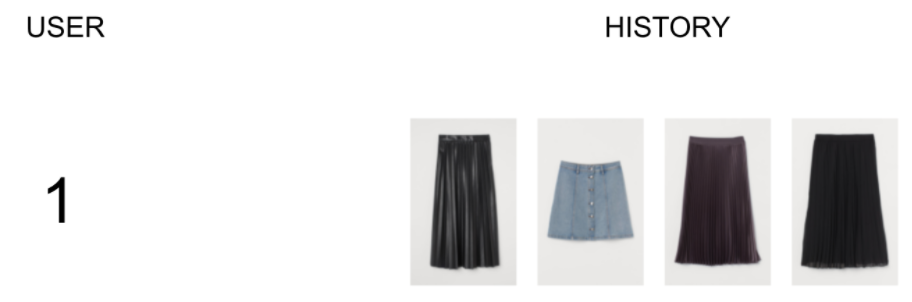
\includegraphics[scale=0.12]{images/dataset/dataset.png} }}%
    % \caption{2 Figures side by side}%
\end{figure}

\column{.5\textwidth} % Right column and width 
\begin{figure}%
    \centering
    \centering{{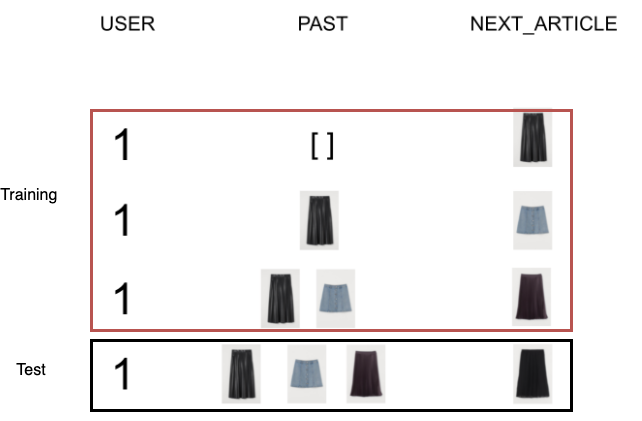
\includegraphics[scale=0.25]{images/dataset/datasetsplit.png} }}%
    % \caption{2 Figures side by side}%
\end{figure}
\end{columns}
\end{frame}

\section{Dataset}

\section{Evaluation}
\begin{frame}{Evaluation}
    
\end{frame}
\section{Models}
\begin{frame}{Models}
\begin{itemize}
    \item AALS - Aproximate Alternative Least Squares (Current method)
    \item Neural Sequencer RNN, LSTM, GRU
    \item Neural Sequencer with attention
    \item Neural Sequencer with transformers
\end{itemize}
\end{frame}

\begin{frame}{Frame Title}
\begin{figure}[!htb]
\minipage{0.32\textwidth}
  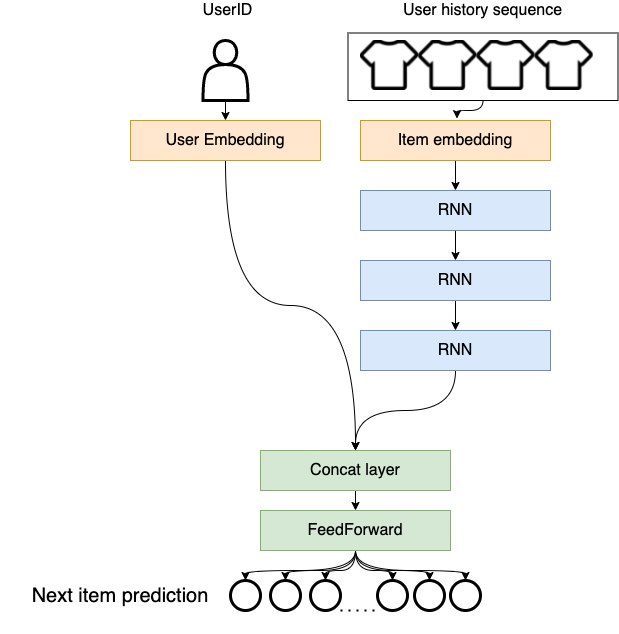
\includegraphics[width=\linewidth]{images/models/RNN.png}
\endminipage\hfill
\minipage{0.32\textwidth}
  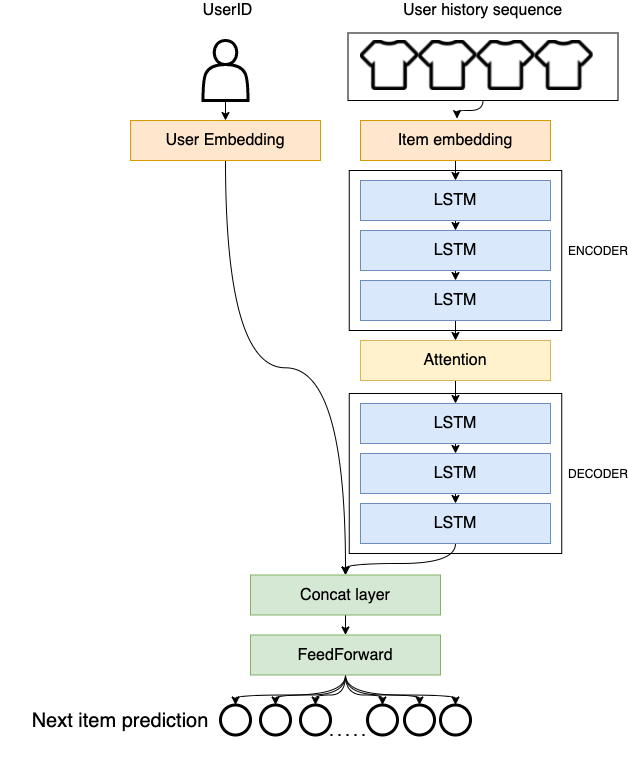
\includegraphics[width=\linewidth]{images/models/Attention.png}
\endminipage\hfill
\minipage{0.32\textwidth}%
  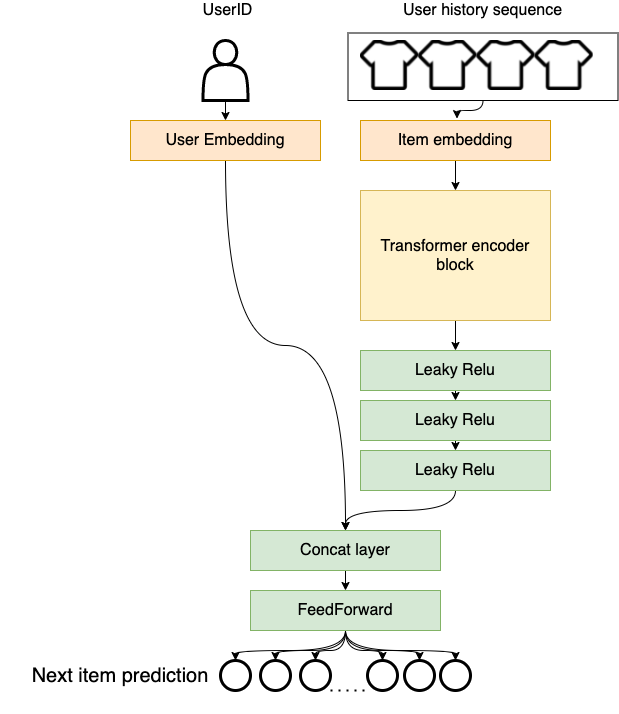
\includegraphics[width=\linewidth]{images/models/Transformer.png}
\endminipage
\end{figure}   
\end{frame}

% \section{Experiments}
% \begin{frame}{Experiments - Models performance}
% \begin{table}[H]
\begin{tabular}{|l|r|r|r|r|r|}
\hline
\multicolumn{1}{|c|}{\textit{Experiments}} & \multicolumn{1}{c|}{\textit{\begin{tabular}[c]{@{}c@{}}HR\\ @14\end{tabular}}} & \multicolumn{1}{c|}{\textit{\begin{tabular}[c]{@{}c@{}}Coverage\\ @14\end{tabular}}} & \multicolumn{1}{c|}{\textit{\begin{tabular}[c]{@{}c@{}}Overlap\\ @14\end{tabular}}} & \multicolumn{1}{c|}{\textit{\begin{tabular}[c]{@{}c@{}}Personalization\\ @14\end{tabular}}} & \multicolumn{1}{c|}{\textit{\begin{tabular}[c]{@{}c@{}}Novelty\\ @14\end{tabular}}} \\ \hline
AALS                                       & 4.42\%                                                                         & 0.24\%                                                                               & {\color[HTML]{333333} \textbf{14.45\%}}                                             & 56.81\%                                                                                     & 7.6                                                                                 \\ \hline
N.S LSTM                                   & \textbf{50.32\%}                                                               & \textbf{8.75\%}                                                                      & {\color[HTML]{333333} 21.54\%}                                                      & \textbf{90.57\%}                                                                            & \textbf{9.88}                                                                       \\ \hline
N.S RNN                                    & 43.94\%                                                                        & 7.68\%                                                                               & {\color[HTML]{333333} 19.84\%}                                                      & 89.87\%                                                                                     & 9.51                                                                                \\ \hline
N.S GRU                                    & 49.00\%                                                                        & 8.04\%                                                                               & {\color[HTML]{333333} 25.94\%}                                                      & 88.03\%                                                                                     & 9.45                                                                                \\ \hline
N.S Attention                              & 47.46\%                                                                        & 7.61\%                                                                               & {\color[HTML]{333333} 19.84\%}                                                      & 89.55\%                                                                                     & 9.44                                                                                \\ \hline
N.S Transformer                            & 44.33\%                                                                        & 7.67\%                                                                               & 21.97\%                                                                             & 86.98\%                                                                                     & 9.36                                                                                \\ \hline
\end{tabular}
\caption{Model results overview} \label{faketable:mul}
\end{table}s
% \end{frame}



\section{Conclusions}
\begin{frame}{Conclusions}

\begin{itemize}
    \item Promising results, maybe too good? Need to be reviewed!
    \item We found a more populated datasource to represent users items preferences than plain transactions.
    \item Around x5 improvement in reco pipeline.
    \item Many possibilities to work with from here on.
\end{itemize}
\end{frame}
%------------------------------------------------
\section{Future work}
\begin{frame}{Future work}
\begin{block}{Dataset}
\begin{itemize}
    \item Cleaning and preprocessing.
    \item Get browsing timestamps within the same day.
    \item Cross market? Split segments? Include transactions?
    \item Weight browsing events, filter on time elapsed.
\end{itemize}
\end{block}

\begin{block}{Article2vec}
\begin{itemize}
\item Pretrained embeddings across markets?
\item Continue exploring visualizations.
\item Create 3d interactive map of embeddings with PCA, T-RNE.
\end{itemize}
\end{block}

\begin{block}{Predicting browsing \& Reco}
\begin{itemize}
    \item Optimize the model, this is a barebones implementation.
    \item We used a very basic model, try attention, multi head attention (transformers) architectures.  \textbf{Huge room for improvement}
    \item Remove the user embedding?
\end{itemize}
\end{block}
\end{frame}

\begin{frame}
\Huge{\centerline{Questions}}
\end{frame}
%----------------------------------------------------------------------------------------

\end{document}